\section{Computer Vision for Fire Detection on UAVs—From Software
to Hardware}

%1
\begin{frame}
    \frametitle{\textit{Computer Vision for Fire Detection on UAVs—From Software
    to Hardware} ~~------~~ Algorithm}

    The UAVs with the payload on them(thermal camera, RGB camrea, etc.), the
    fire detection algorithms and the open data set of the forest fire are
    introduced.

    \begin{itemize}
        \item \textbf{Fire Detection Framework:}
            \begin{itemize}
                \item Preprocessing: reduce the noise, normalization, etc.
                \item Segmentation: based on the colors, motion or even intensities.
                \item Fire Detection and Feature Extracting: Feature ~ is aimed to
                    identify the key points of interest.
            \end{itemize}
        \item Traditional Methods:
            \begin{itemize}
                \item Optimal Residual Network-Based Features Extraction algorithm (O-RNBFE)
                    for feature extraction and a Latent Variable Support Vector Machine (LVSVM)
                    for classification.
                \item descriptor: Gray Level Co-occurrence Matrix (GLCM),
                    Spatial and Geometric Histograms (SGH) descriptor, Local
                    Binary Pattern (LBP)
            \end{itemize}

        \item But the \textbf{Deep Learning-based methods} greatly simplify the
            segmentation and feature extracting.
            \begin{itemize}
                \item VGG-16, Resnet34, Resnet50, U-Net and MobileNet
                \item Faster-RCNN
                \item YOLO
                \item Mobilenet(lightweight framework, see also YOLO-fast,
                    YOLO-tiny and Mobilenet-SSD)
                \item SSD(Single Shot MultiBox Detector)
            \end{itemize}

        \item \textbf{Softwares:}
            \begin{itemize}
                \item ROS
                \item OpenCV
                \item DroneDeploy+PIX4D
            \end{itemize}
    \end{itemize}
\end{frame}

%2
\begin{frame}
    \frametitle{\textit{Computer Vision for Fire Detection on UAVs—From Software
    to Hardware} ~~------~~ Hardware}
    \begin{itemize}
        \item UAVs classifications and Trends:
            \begin{figure}[H]
                \centering
                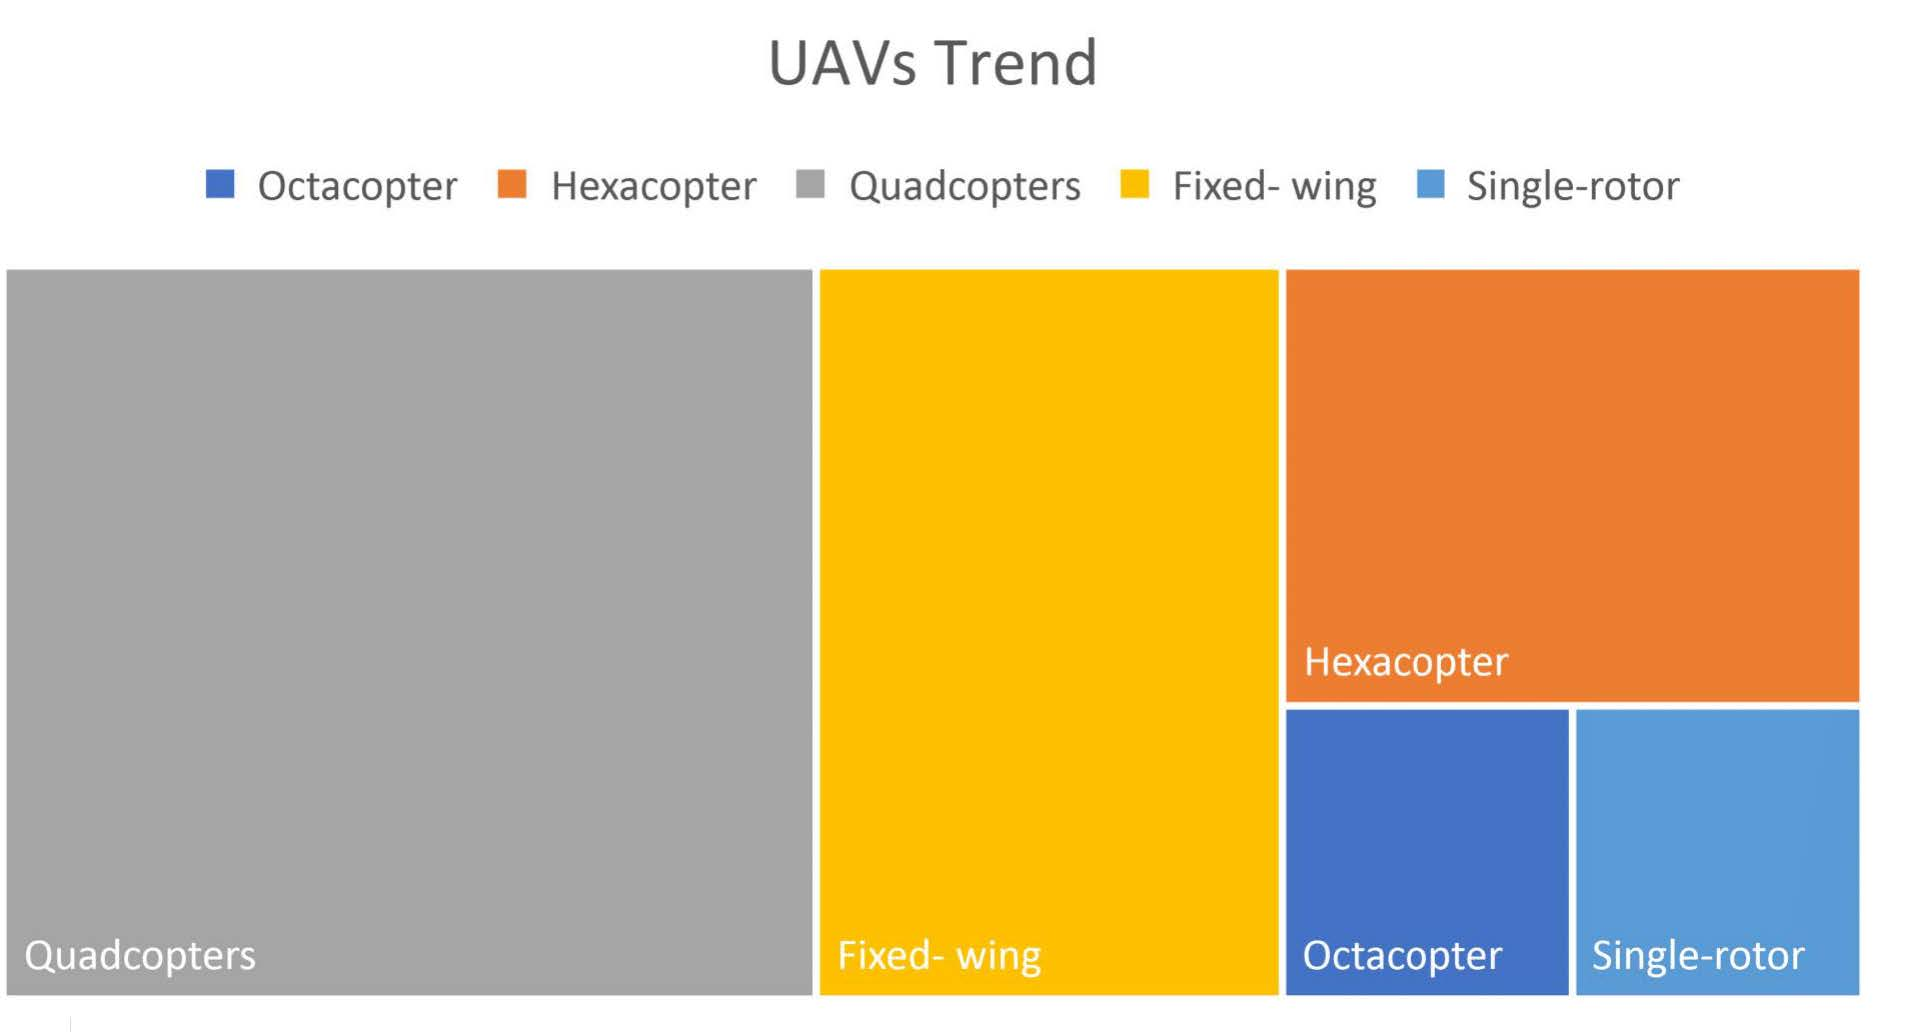
\includegraphics[width=0.7\textwidth]{./imgs/UAV_Trends}
            \end{figure}
        \item Cameras: Visible Spectrum, IR System, Multispectral/Hyperspectral
        \item Platform: Raspberry, ARM, FPGA, IMU, GPS, GNSS, On-board Computer.
    \end{itemize}

\end{frame}
